\documentclass[11pt, a4paper, twoside]{article}   	% use "amsart" instead of "article" for AMSLaTeX format

\usepackage{geometry}                		% See geometry.pdf to learn the layout options. There are lots.
\usepackage{pdfpages}
\usepackage{caption}
\usepackage{minted}
\usepackage[german]{babel}			% this end the next are needed for german umlaute
\usepackage[utf8]{inputenc}
\usepackage{color}
\usepackage{graphicx}
\usepackage{titlesec}
\usepackage{fancyhdr}
\usepackage{lastpage}
\usepackage{hyperref}
\usepackage[autostyle=false, style=english]{csquotes}
\usepackage{mathtools}
\usepackage{tabularx}
% http://www.artofproblemsolving.com/wiki/index.php/LaTeX:Symbols#Operators
% =============================================
% Layout & Colors
% =============================================
\geometry{
   a4paper,
   total={210mm,297mm},
   left=20mm,
   right=20mm,
   top=20mm,
   bottom=30mm
 }	

\definecolor{myred}{rgb}{0.8,0,0}
\definecolor{mygreen}{rgb}{0,0.6,0}
\definecolor{mygray}{rgb}{0.5,0.5,0.5}
\definecolor{mymauve}{rgb}{0.58,0,0.82}

\setcounter{secnumdepth}{4}


% the default java directory structure and the main packages
\newcommand{\srcDir}{../src/}
\newcommand{\imageDir}{./images/}
% =============================================
% Code Settings
% =============================================
\newenvironment{code}{\captionsetup{type=listing}}{}
\newmintedfile[mSourceFile]{matlab}{
	linenos=true, 
	frame=single, 
	breaklines=true, 
	tabsize=2,
	numbersep=5pt,
	xleftmargin=10pt,
	baselinestretch=1,
	fontsize=\footnotesize
}
\newmintinline[mInlineSource]{matlab}{}
\newminted[mSource]{matlab}{
	breaklines=true, 
	tabsize=2,
	autogobble=true,
	breakautoindent=false
}
% =============================================
% Page Style, Footers & Headers, Title
% =============================================
\title{Übung 1}
\author{Thomas Herzog}

\lhead{Übung 1}
\chead{}
\rhead{
\includegraphics[scale=0.10]{FHO_Logo_Students.jpg}}

\lfoot{S1610454013}
\cfoot{}
\rfoot{ \thepage / \pageref{LastPage} }
\renewcommand{\footrulewidth}{0.4pt}
% =============================================
% D O C U M E N T     C O N T E N T
% =============================================
% =============================================
% 2016.10.13: 1 
% 2016.10.14: 2
% =============================================

\pagestyle{fancy}
\begin{document}
\setlength{\headheight}{15mm}
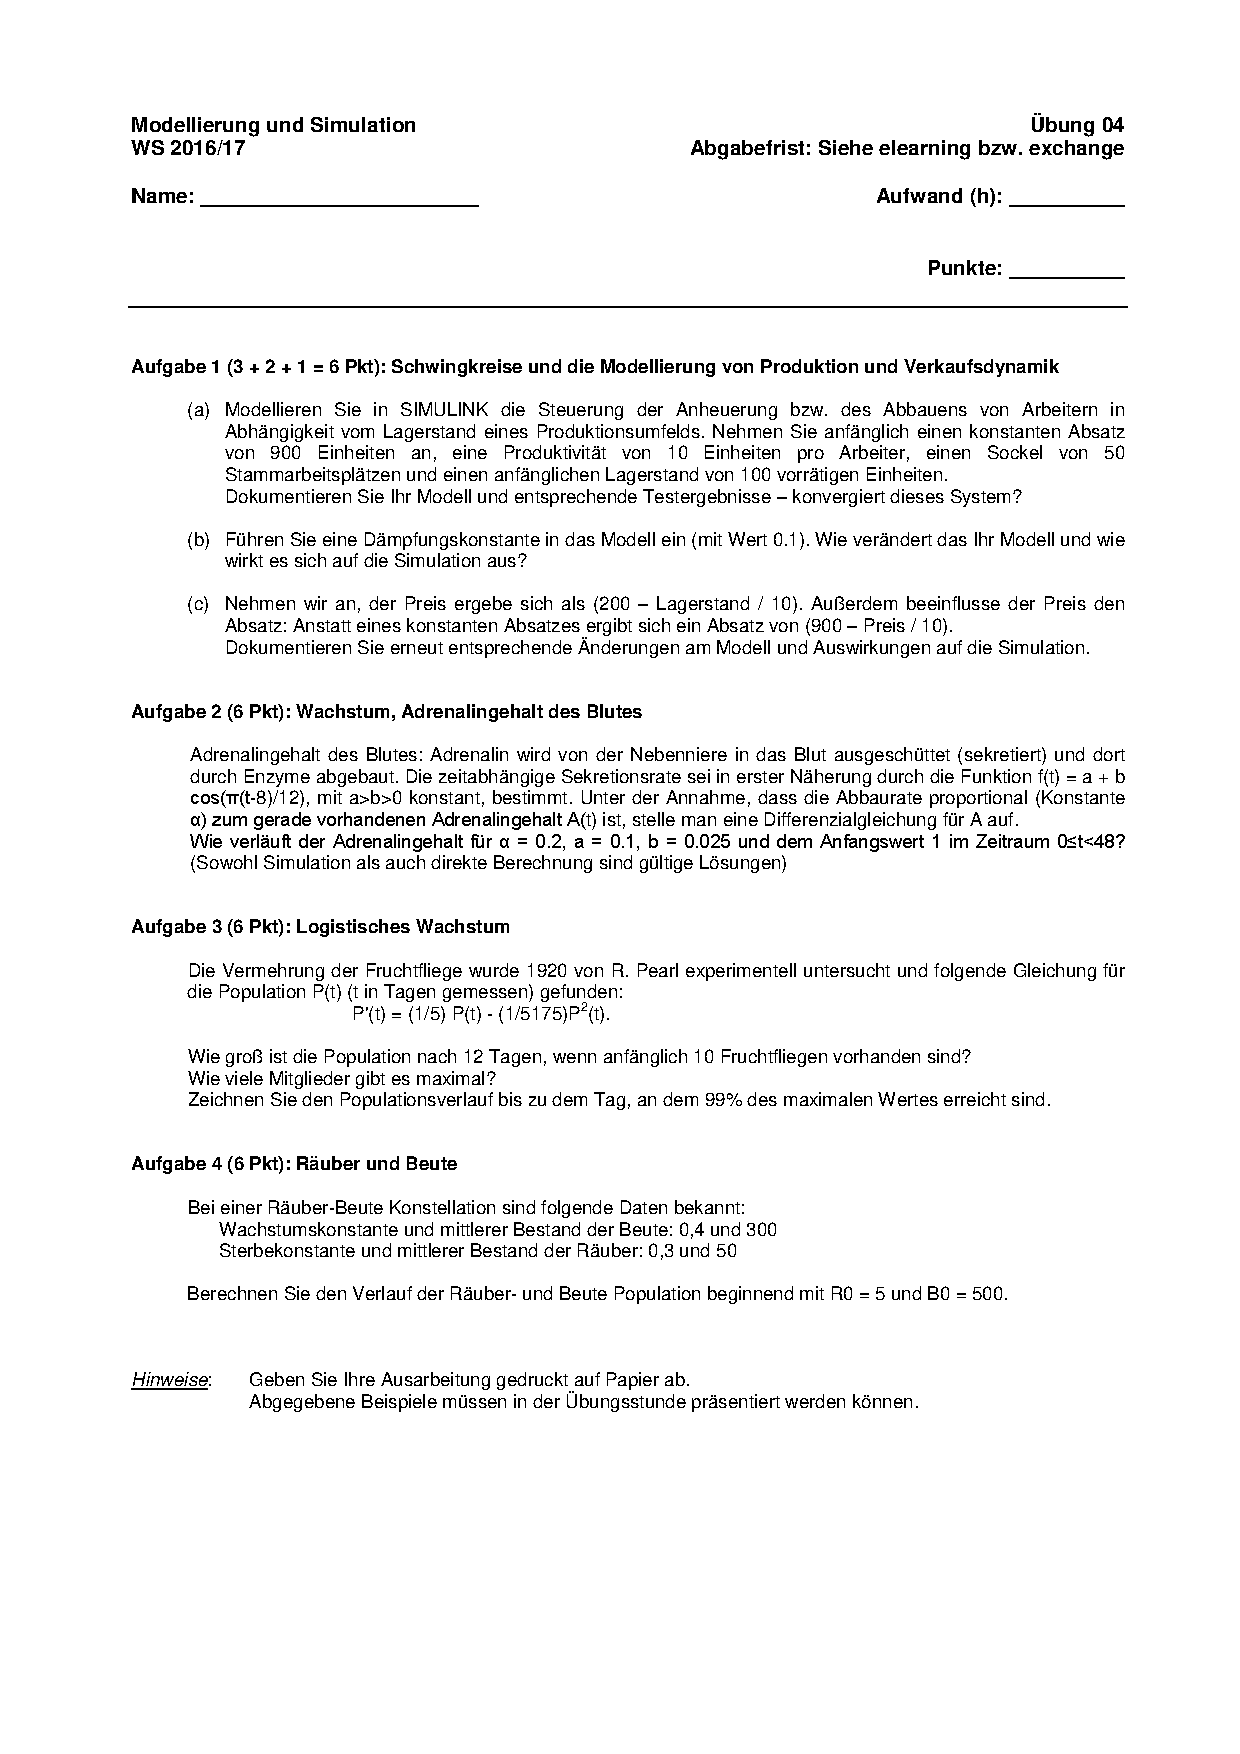
\includepdf[pages={1}]{Uebungszettel04.pdf}

\section{Schwingkreise und Verkaufsdynamik}

\subsection{a}
\subsection{b}
\subsection{c}
$
 f(t): a + b + cos(\pi(t-8)/12), \hspace{5pt} mit \hspace{10pt} a>b>0.
 \newline\newline
 A(t): A_0 * \alpha^t 
$


\section{Adrenalingehalt des Blutes}
\begin{code}
	\caption{Skript für die diskrete Berechnung des Verlaufs}
	\mSourceFile{\srcDir/growAdrenalin.m}
	\label{source:2-script}
\end{code}
\ \newpage

\begin{figure}[h]
\centering
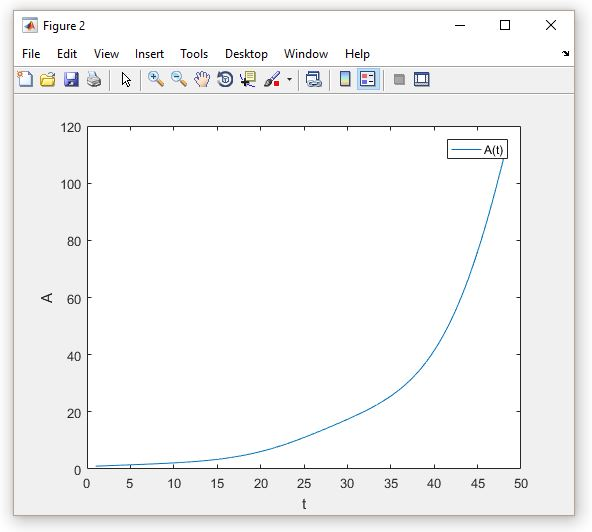
\includegraphics[scale=1]{\imageDir/2-test.JPG}
\caption{Verlauf des Adrenalingehalts}
\label{fig:1-c-modell}
\end{figure}
\ \newline
Der Verlauf wurde diskret berechnet, da die Abbaurate proportional zum aktuellen Adrenalingehalt ist.
\newpage
\section{Logistisches Wachstum}
\begin{code}
	\caption{Skript für die kontinuierliche Berechnung des Verlaufs}
	\mSourceFile{\srcDir/logisticFlys.m}
	\label{source:3-script}
\end{code}
\ \newpage
\begin{figure}[h]
	\centering
	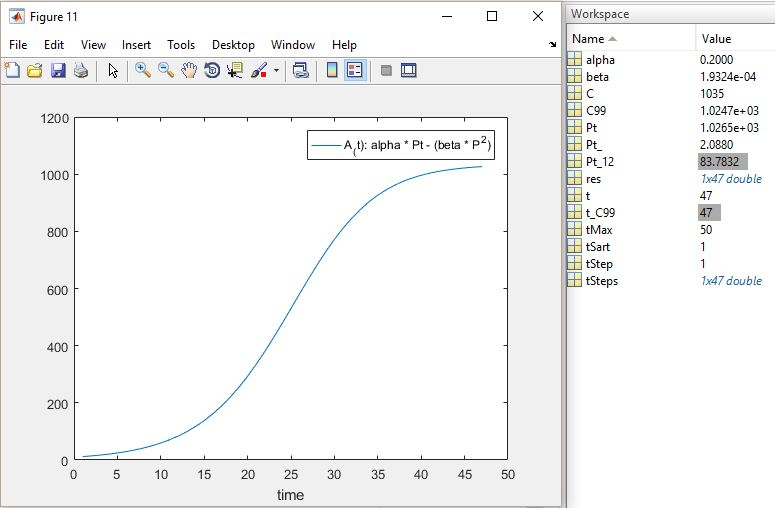
\includegraphics[scale=1,angle=90]{\imageDir/3-test.JPG}
	\caption{t\_99=47, Pt\_12=83.7832}
	\label{fig:3-test}
\end{figure}
\section{Logistisches Wachstum}
\begin{code}
	\caption{Skript für die kontinuierliche Berechnung des Verlaufs}
	\mSourceFile{\srcDir/predatorPrey.m}
	\label{source:3-script}
\end{code}
\ \newpage
\begin{figure}[h]
	\centering
	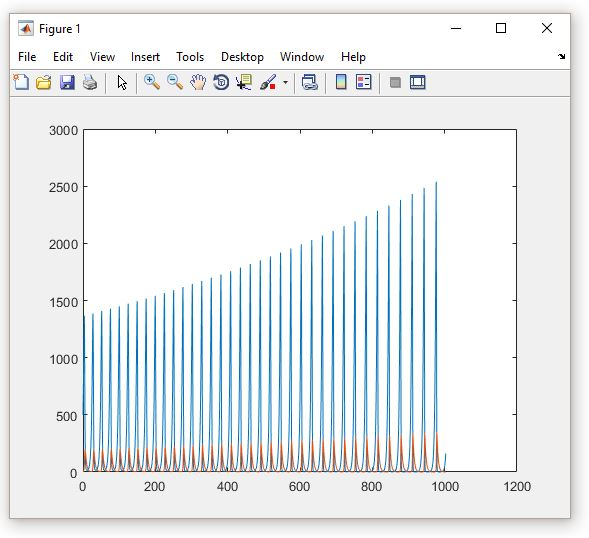
\includegraphics[scale=1]{\imageDir/4-test.JPG}
	\caption{Verlauf}
	\label{fig:3-test}
\end{figure}

\end{document}
